\chapter{Resultate}
In diesem Kapitel befinden sich alle Resultate thematisch zusammengefasst.

\section{CrossDomain}
Dieses Experiment dient zur Beantwortung der Kernfrage dieser Arbeit. Es wurde das Experiment V8 durchgeführt um die Entwicklung des F1 Score zu sehen, wenn nur mit Daten der Zieldomäne trainiert wird. Somit enthält das Experiment V8 keine domänenfremde Daten beim trainieren.

Dagegen wurde das Experiment V6 durchgeführt, mit den Konfigurationen wie im Kapitel 5.3.3 beschrieben.

Die resultierenden F1 (vgl. 5.1) Score sind in den Grafiken \ref{fig:Results V6 und V8} ersichtlich. Der blaue Graph steht für die Experimentreihe V8 und somit der Baseline. Der gelbe Graph repräsentiert die Experimente V6 CrossDomain.
\begin{figure}[H]
	\centering
	\subfigure[V6 gegen V8 auf MPQ mit news Emeddings]{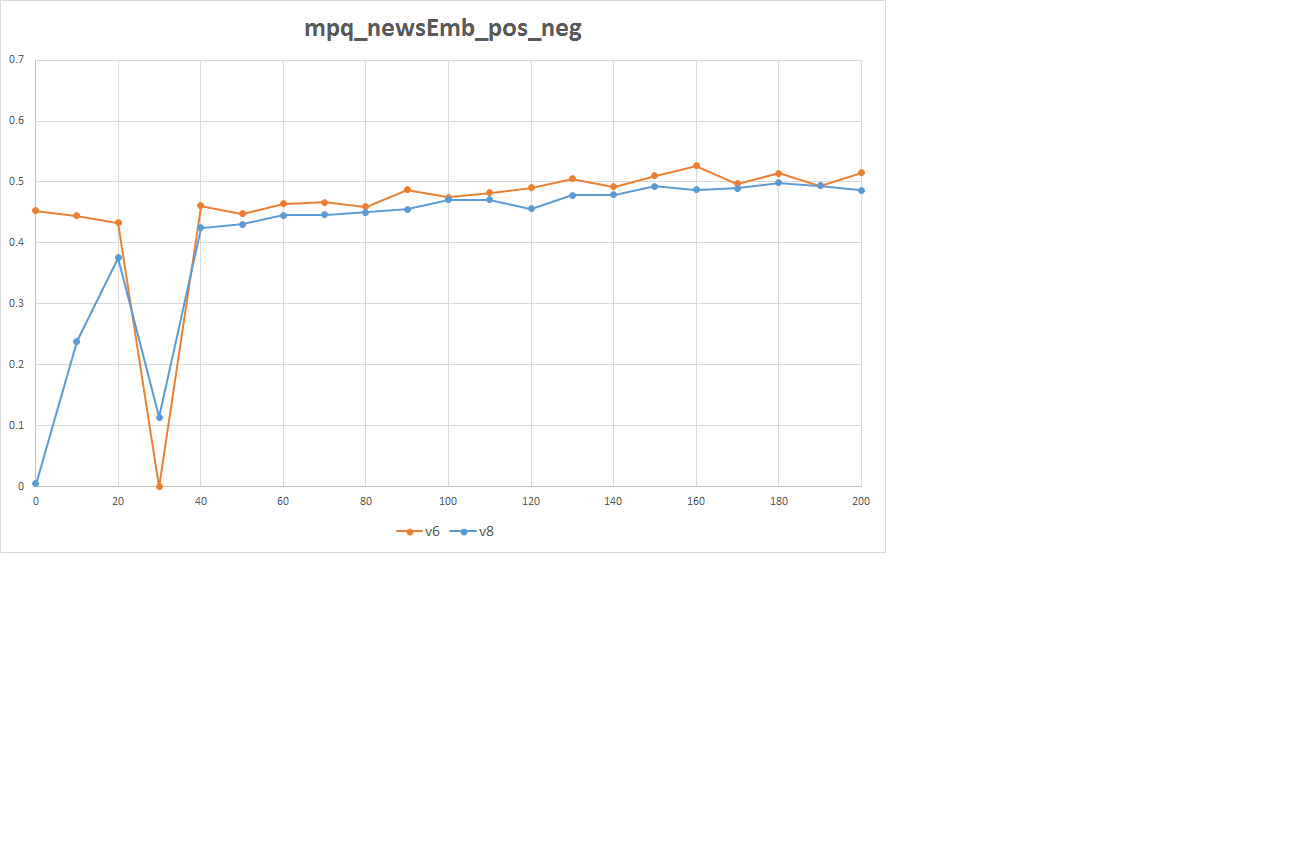
\includegraphics[width=0.49\textwidth]{img/CrossDomain_V6-V8_MPQ_newsEmb.png}}
	\subfigure[V6 gegen V8 auf MPQ mit tweets Emeddings]{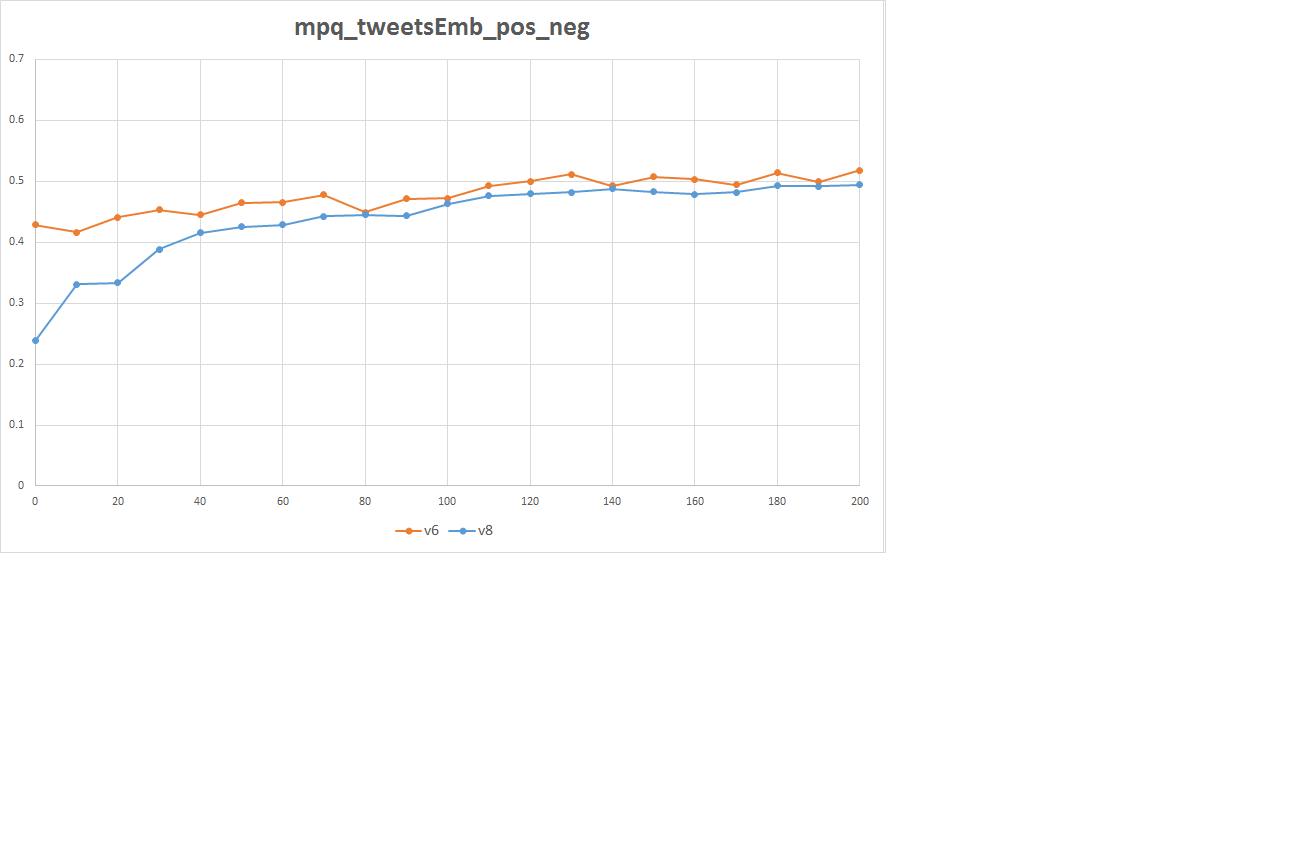
\includegraphics[width=0.49\textwidth]{img/CrossDomain_V6-V8_MPQ_tweetsEmb.png}}
	\subfigure[V6 gegen V8 auf SemEval mit news Emeddings]{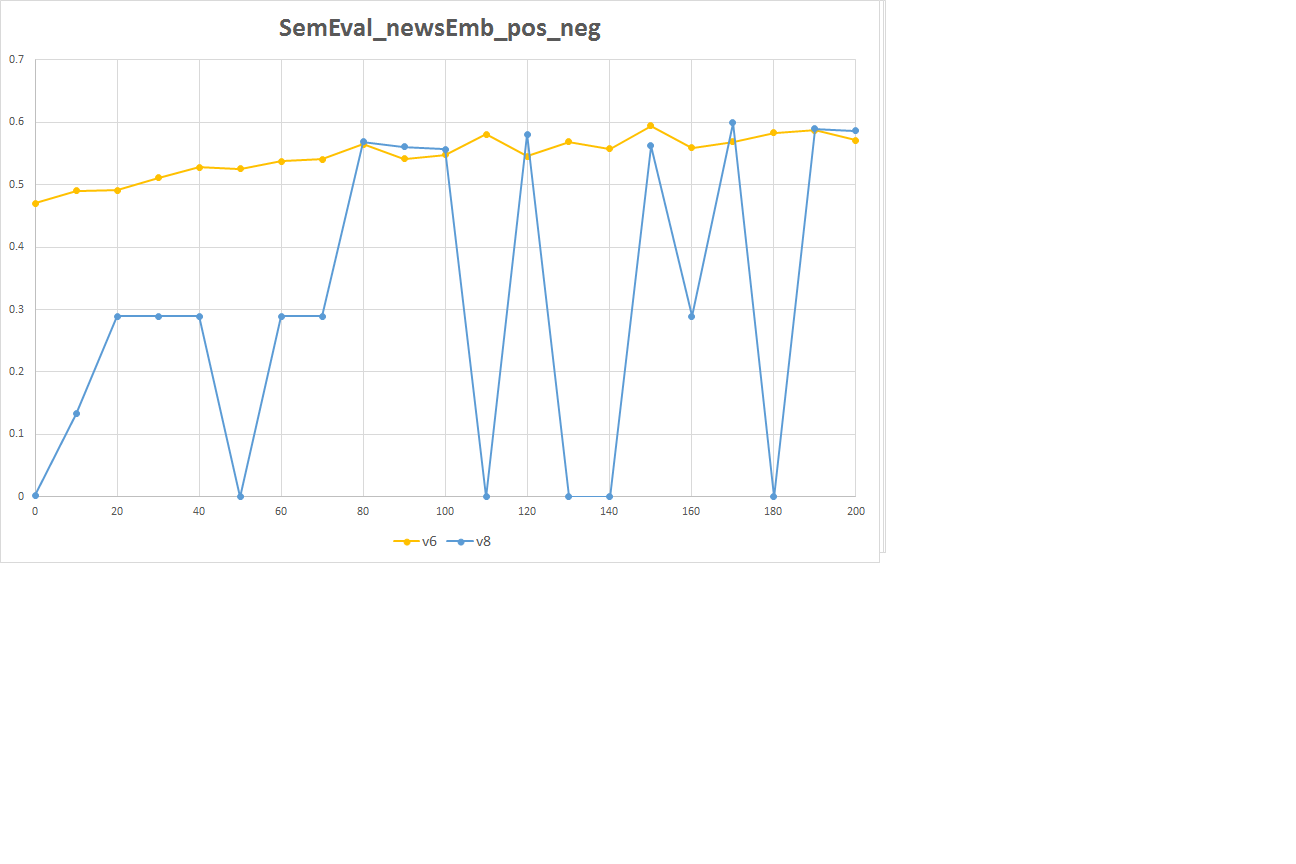
\includegraphics[width=0.49\textwidth]{img/CrossDomain_V6-V8_SemEval_newsEmb.png}}
	\subfigure[V6 gegen V8 auf SemEval mit tweets Emeddings]{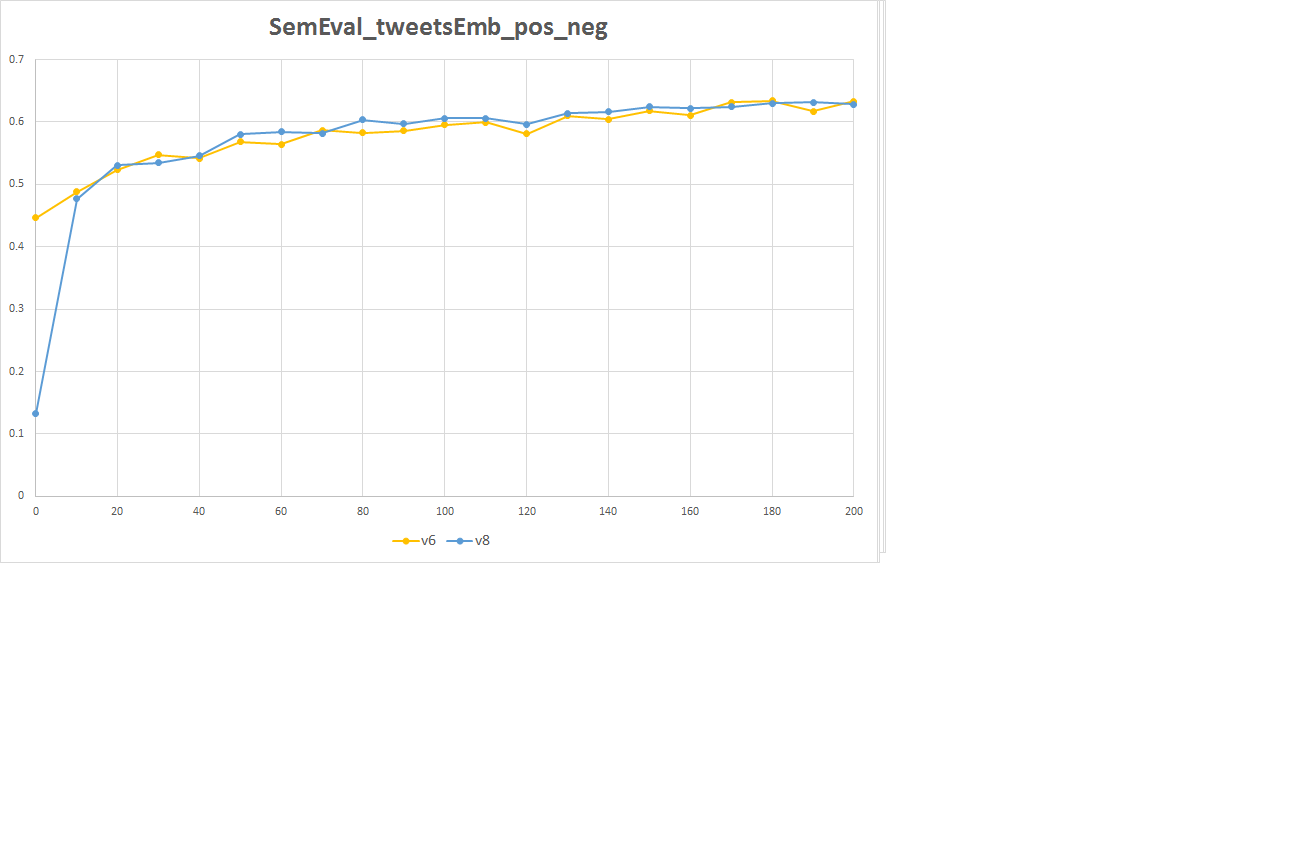
\includegraphics[width=0.49\textwidth]{img/CrossDomain_V6-V8_SemEval_tweetsEmb.png}}
	\caption{CrossDomain, F1 Score V6 und V8}
	\label{fig:Results V6 und V8}
\end{figure}

%TODO Baseline erklärung/refernzierung?!

\section{Distant-Phase}
In diesem Kapitel befindet sich die Ergebnisse der Experimente mit und ohne Distant Phase. Es wurden jeweils die gleichen Experimente mit und ohne einer Distant-Phase durchgeführt. Dabei gilt folgende Namensgebung:
\begin{itemize}  
	\item V10 entspricht V6 mit Distant-Phase
	\item V11 entspricht V7 mit Distant-Phase
	\item V12 entspricht V8 mit Distant-Phase
\end{itemize}
Dabei sind die blauen Graphen jeweils die Experimente ohne Distant-Phase und die gelben Graphen diejenigen mit der Distant-Phase.

\begin{figure}[H]
	\centering
	\subfigure[V6 gegen V10 auf MPQ mit news Emeddings]{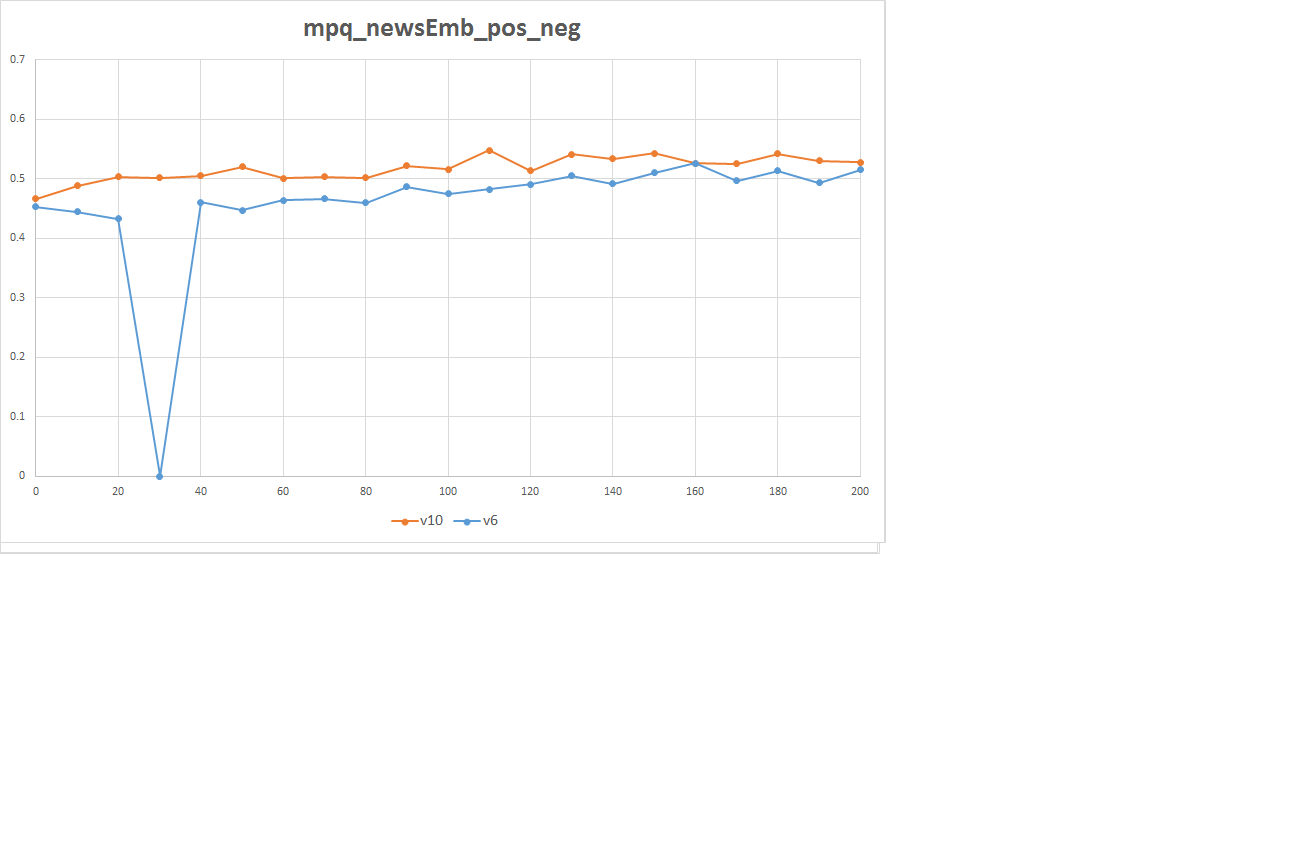
\includegraphics[width=0.49\textwidth]{img/DistantPhase_V6-V10_MPQ_newsEmb.png}}
	\subfigure[V6 gegen V10 auf MPQ mit tweets Emeddings]{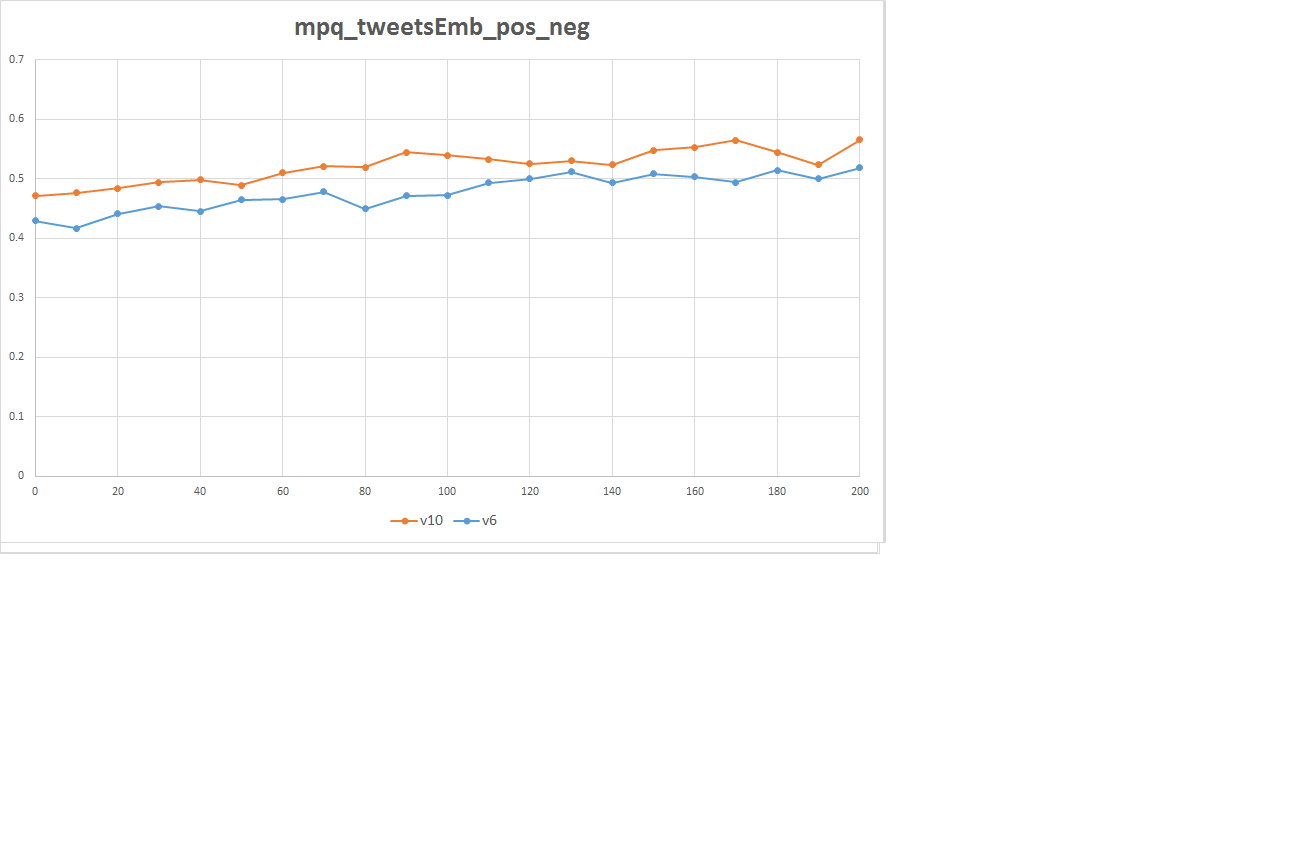
\includegraphics[width=0.49\textwidth]{img/DistantPhase_V6-V10_MPQ_tweetsEmb.png}}
	\subfigure[V6 gegen V10 auf SemEval mit news Emeddings]{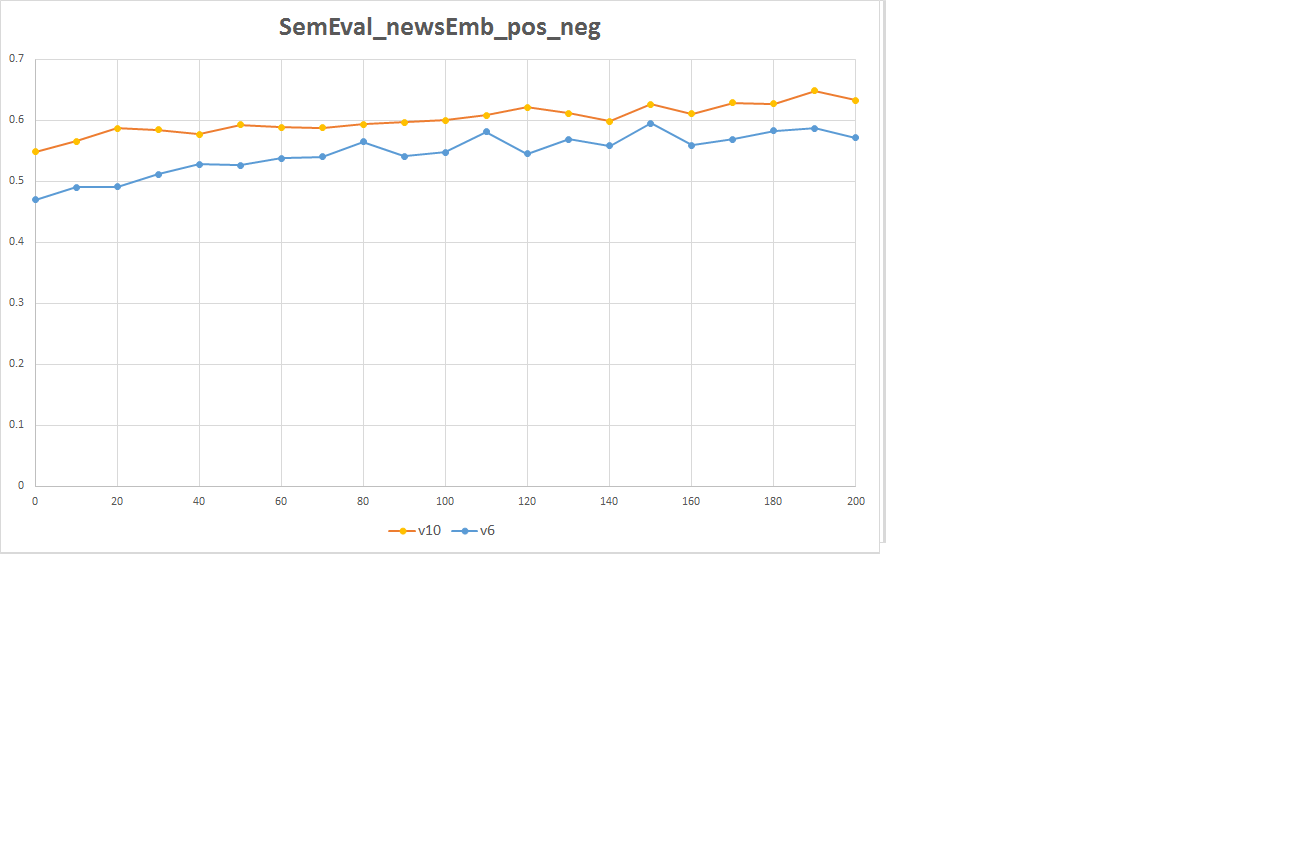
\includegraphics[width=0.49\textwidth]{img/DistantPhase_V6-V10_SemEval_newsEmb.png}}
	\caption{Distant Phase, F1 Score V6 und V10}
	\label{fig:Results V6 und V10}
\end{figure}

\begin{figure}[H]
	\centering
	\subfigure[V8 gegen V12 auf MPQ mit news Emeddings]{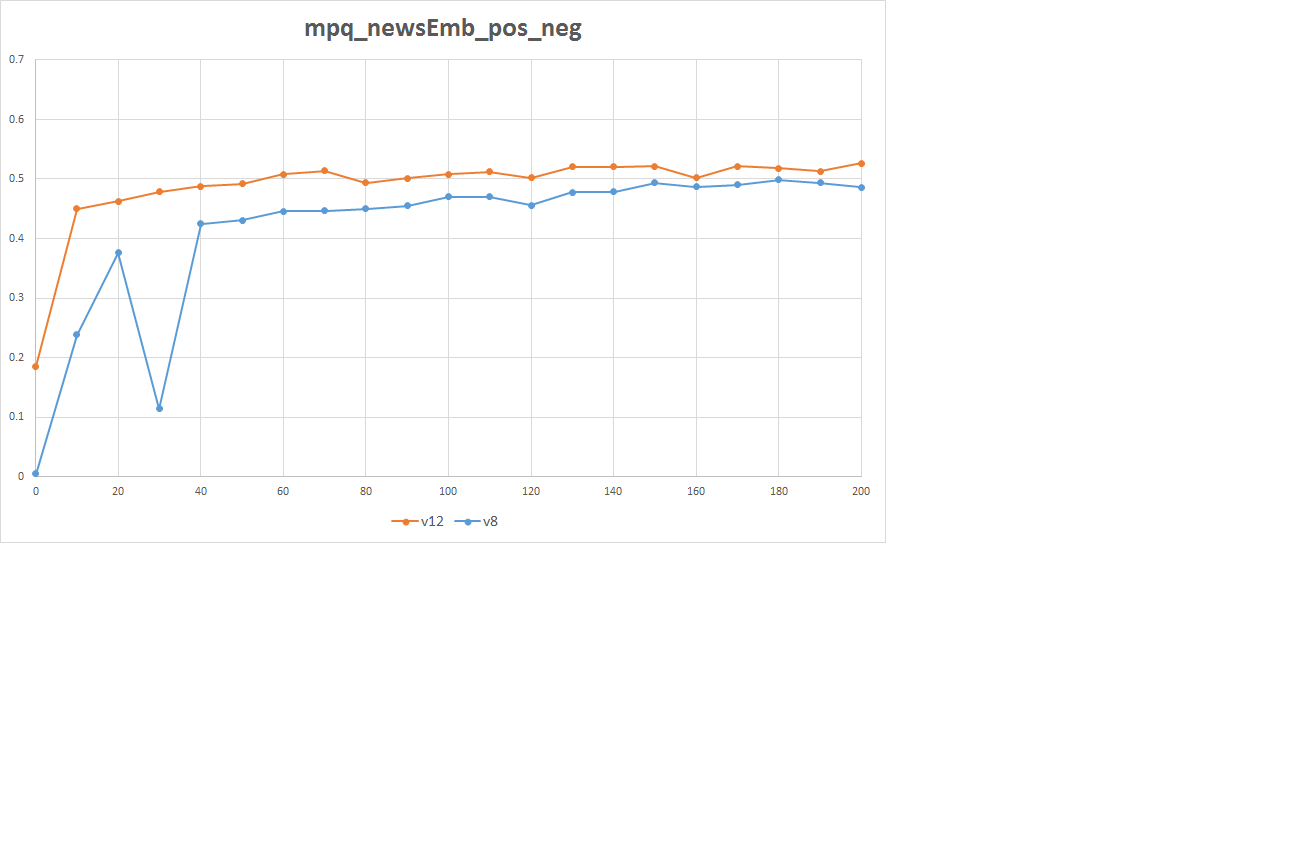
\includegraphics[width=0.49\textwidth]{img/DistantPhase_V8-V12_MPQ_newsEmb.png}}
	\subfigure[V8 gegen V12 auf MPQ mit tweets Emeddings]{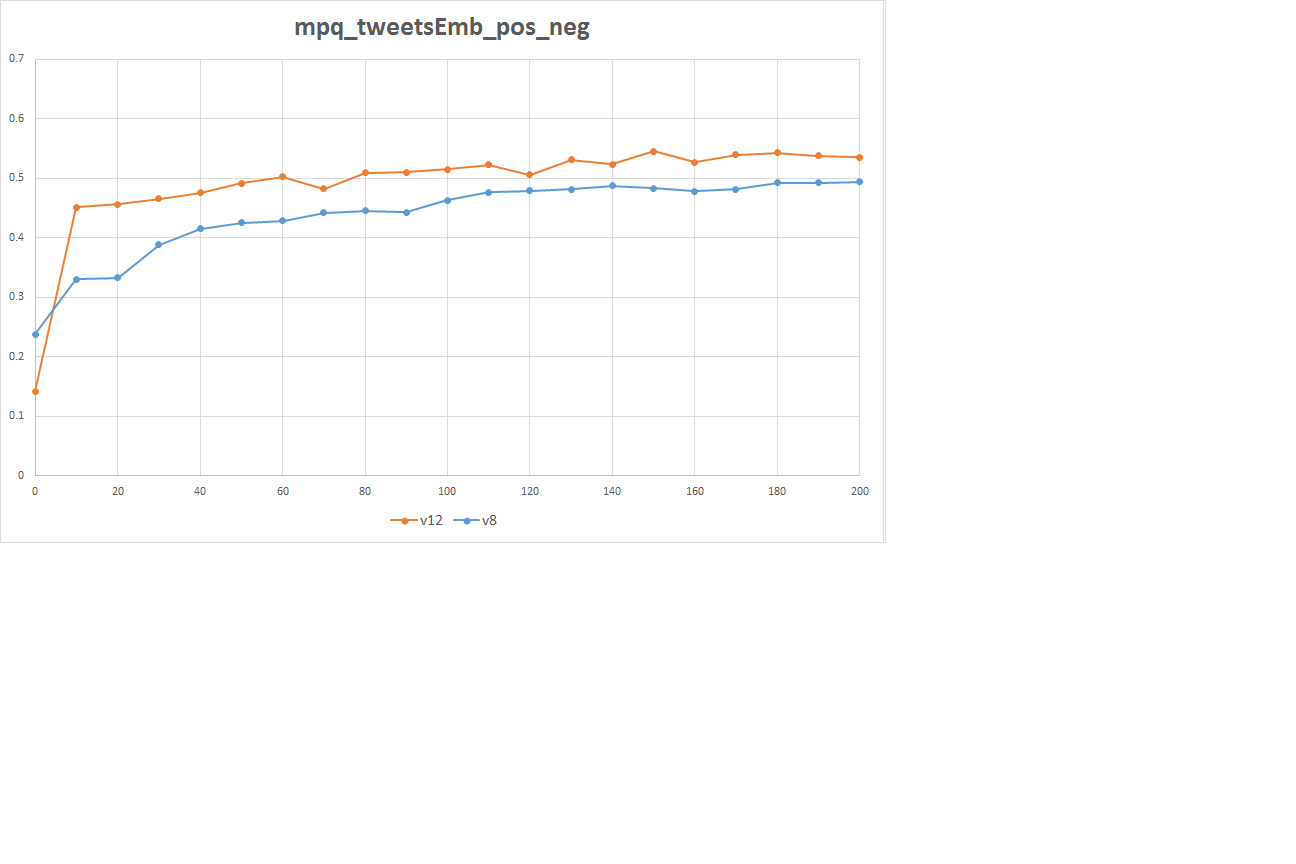
\includegraphics[width=0.49\textwidth]{img/DistantPhase_V8-V12_MPQ_tweetsEmb.png}}
	\subfigure[V8 gegen V12 auf SemEval mit news Emeddings]{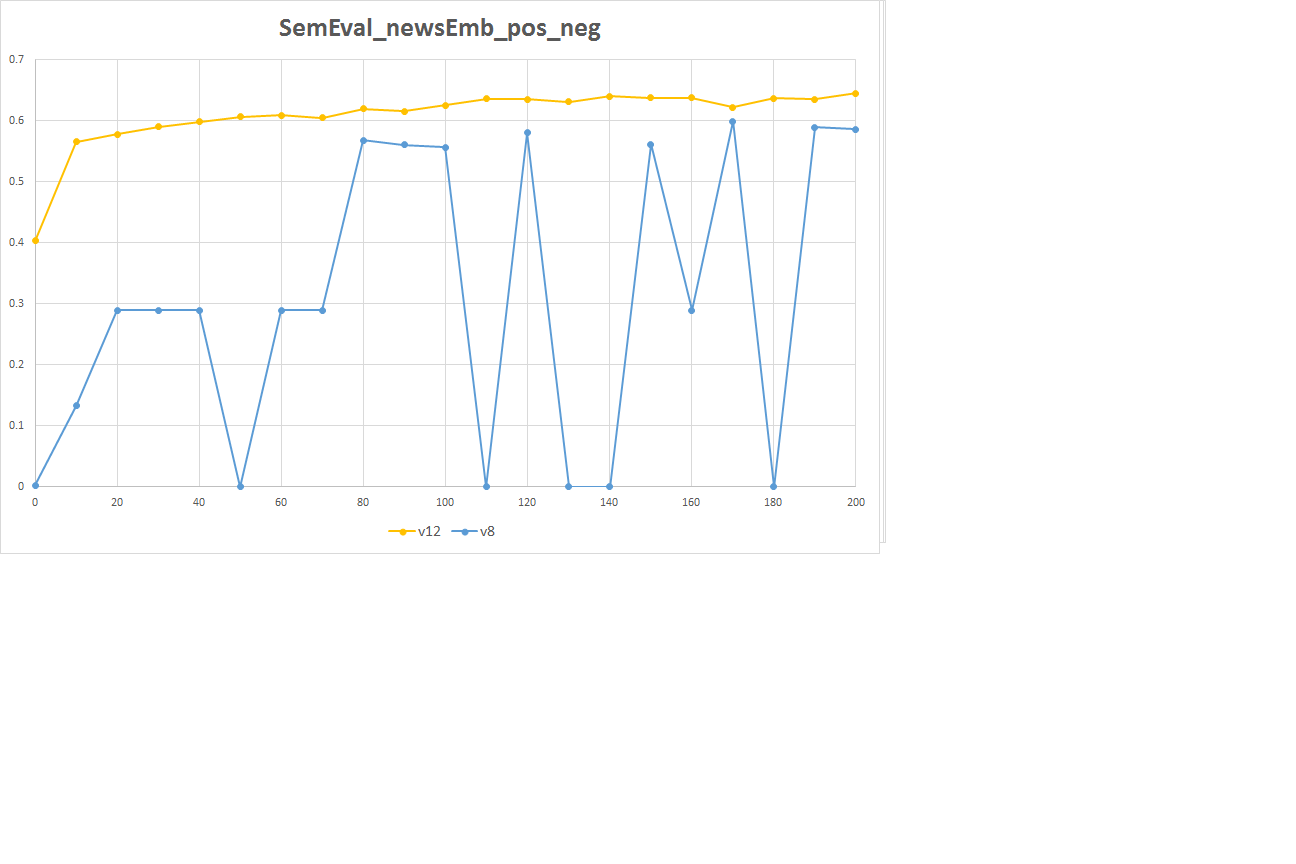
\includegraphics[width=0.49\textwidth]{img/DistantPhase_V8-V12_SemEval_newsEmb.png}}
	\subfigure[V8 gegen V12 auf SemEval mit tweets Emeddings]{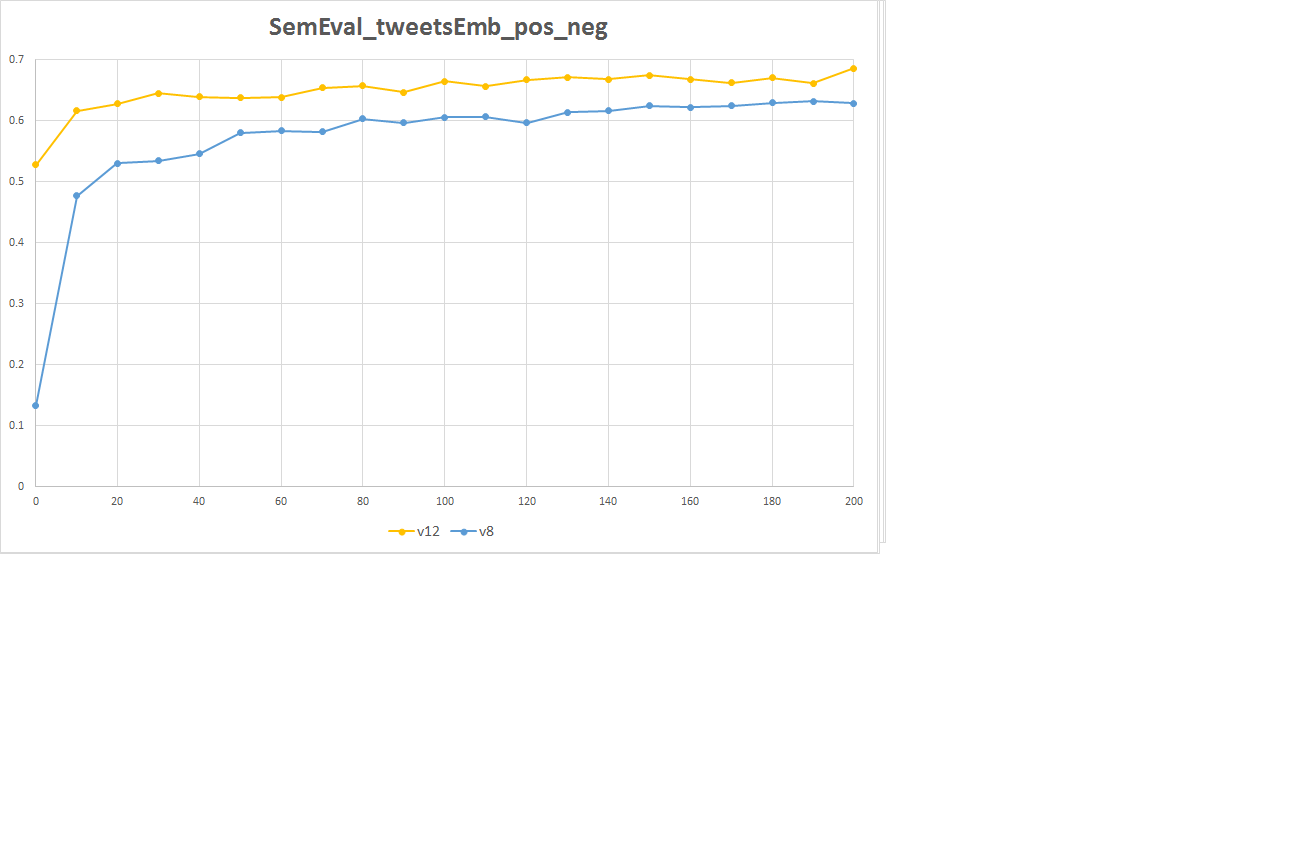
\includegraphics[width=0.49\textwidth]{img/DistantPhase_V8-V12_SemEval_tweetsEmb.png}}
	\caption{Distant Phase, F1 Score V8 und V12}
	\label{fig:Results V8 und V12}
\end{figure}

\section{Word-Embeddings}
Alle obigen Experimente wurden mit 2 verschiedenen Word-Embeddings durchgeführt. Die Embeddings basieren auf unterschiedlichen Domänen.
News Embeddings basieren auf News Texten, welche durchschnittlich länger sind (vgl. Kapitel Daten....analyse länge der Texte news) und grammatikalisch auf Korrektheit geprüft wurden.
Tweets Embeddings sind eher kürzere Sätze (vgl. Kapitel Daten analyse testlänge tweets und stellen nicht den Anspruch, grammatikalisch korrekt zu sein.
%TODO Referenz auf Länge der Sätze, im Kapitel Daten
Jeweils die blauen Graphen repräsentieren die Ergebnisse mit News Embeddings und die gelben Graphen derjenigen mit den Tweets Embeddings.

\begin{figure}[H]
	\centering
	\subfigure[V6 auf MPQ mit news Emeddings]{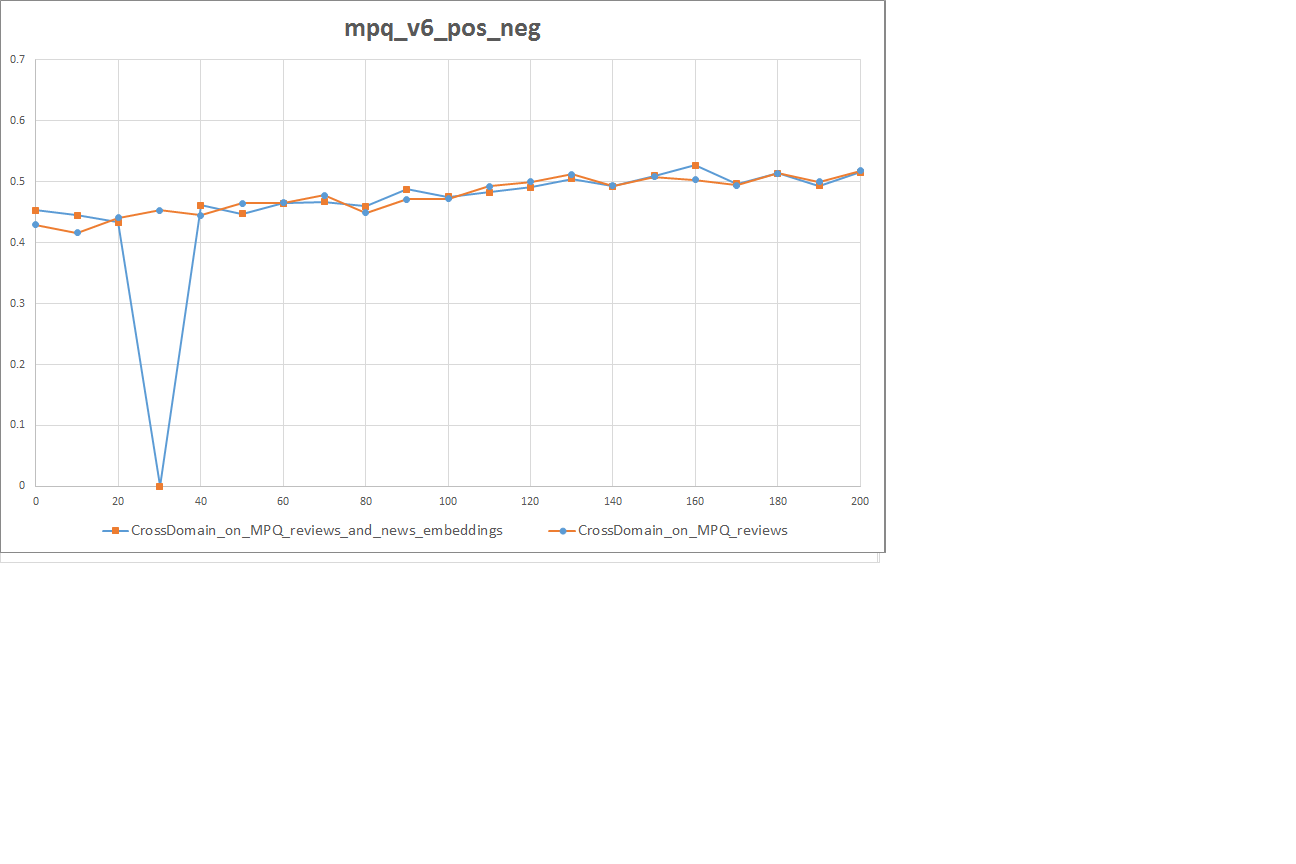
\includegraphics[width=0.49\textwidth]{img/Embeddings_V6_MPQ.png}}
	\subfigure[V6 auf SemEval mit tweets Emeddings]{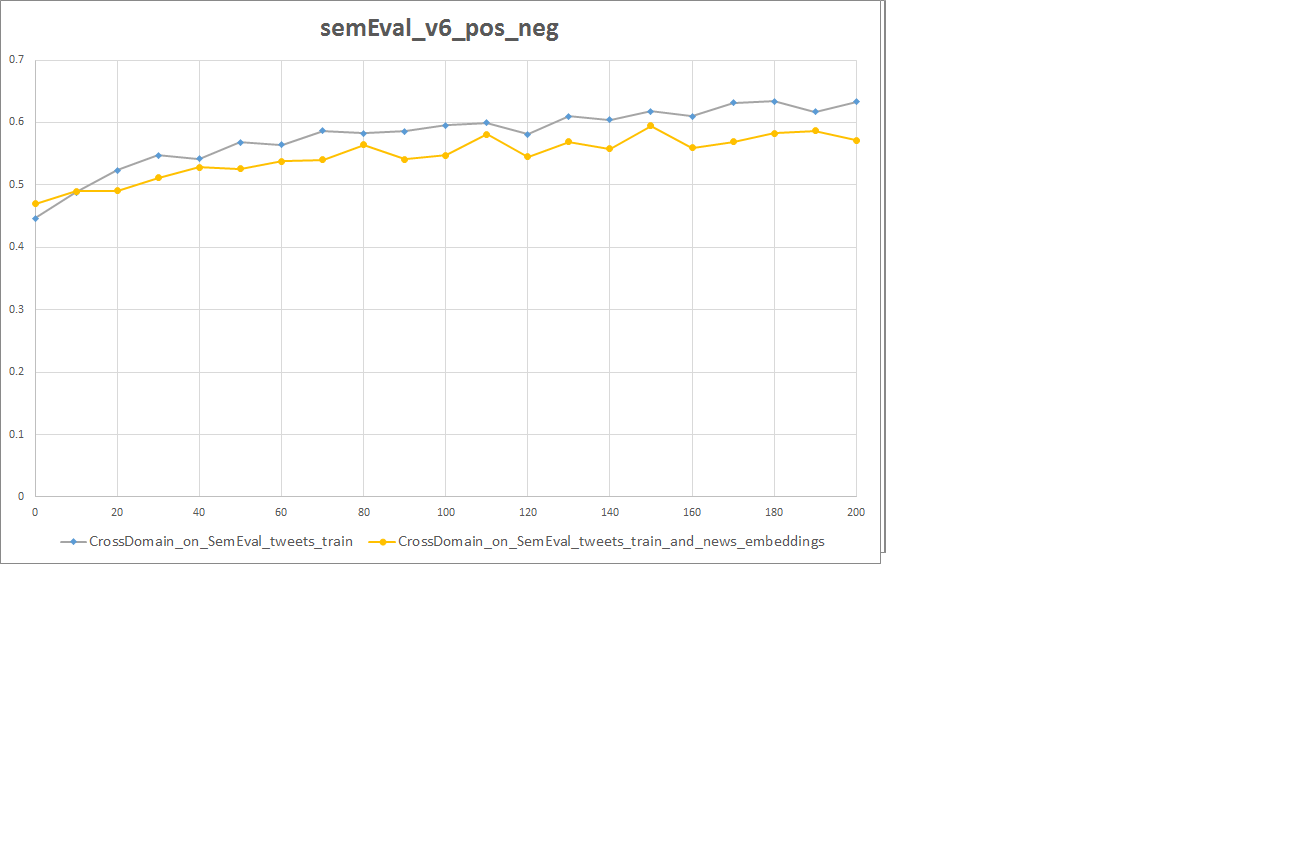
\includegraphics[width=0.49\textwidth]{img/Embeddings_V6_SemEval.png}}
	\caption{Word-Embeddings, F1 Score V6}
	\label{fig:Results V6}
\end{figure}

\begin{figure}[H]
	\centering
	\subfigure[V8 auf MPQ mit news Emeddings]{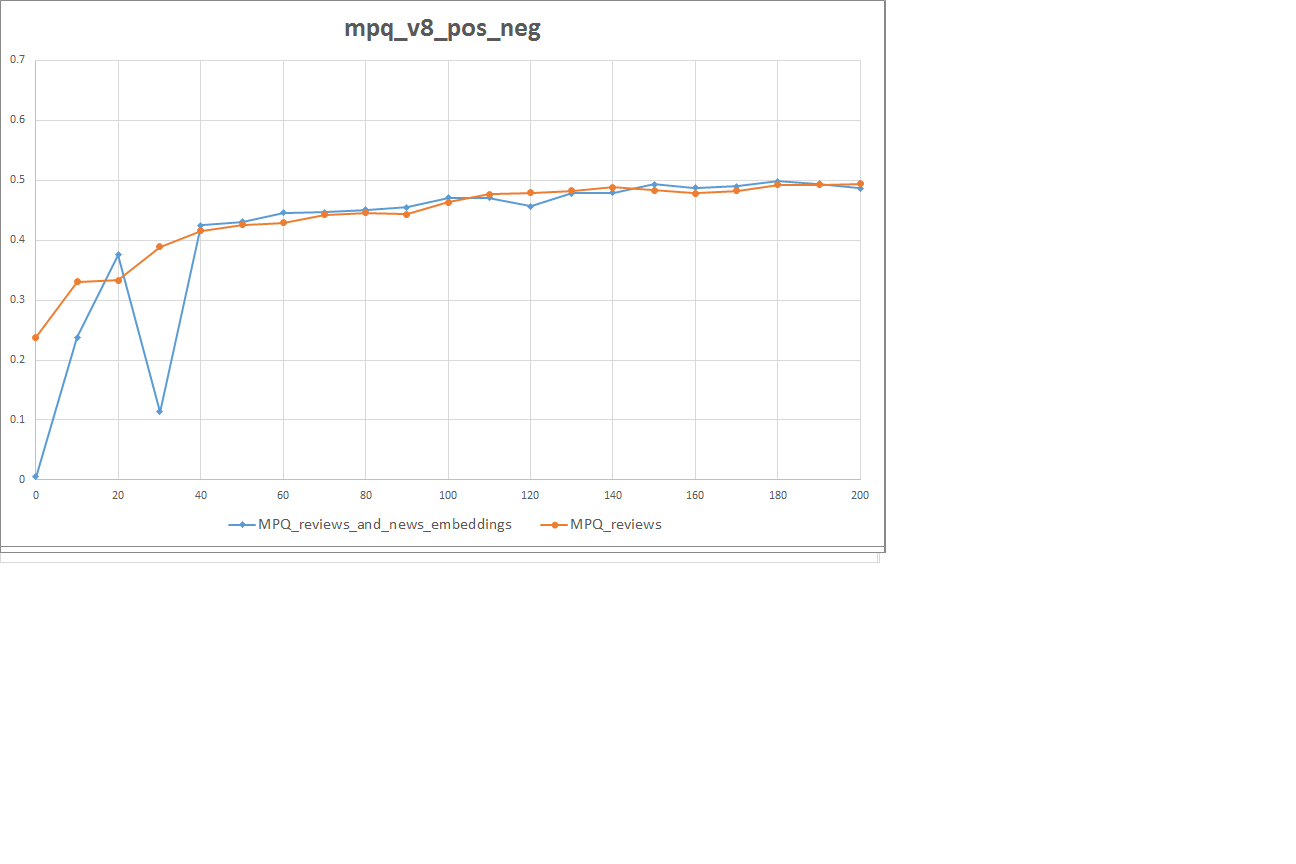
\includegraphics[width=0.49\textwidth]{img/Embeddings_V8_MPQ.png}}
	\subfigure[V8 auf SemEval mit tweets Emeddings]{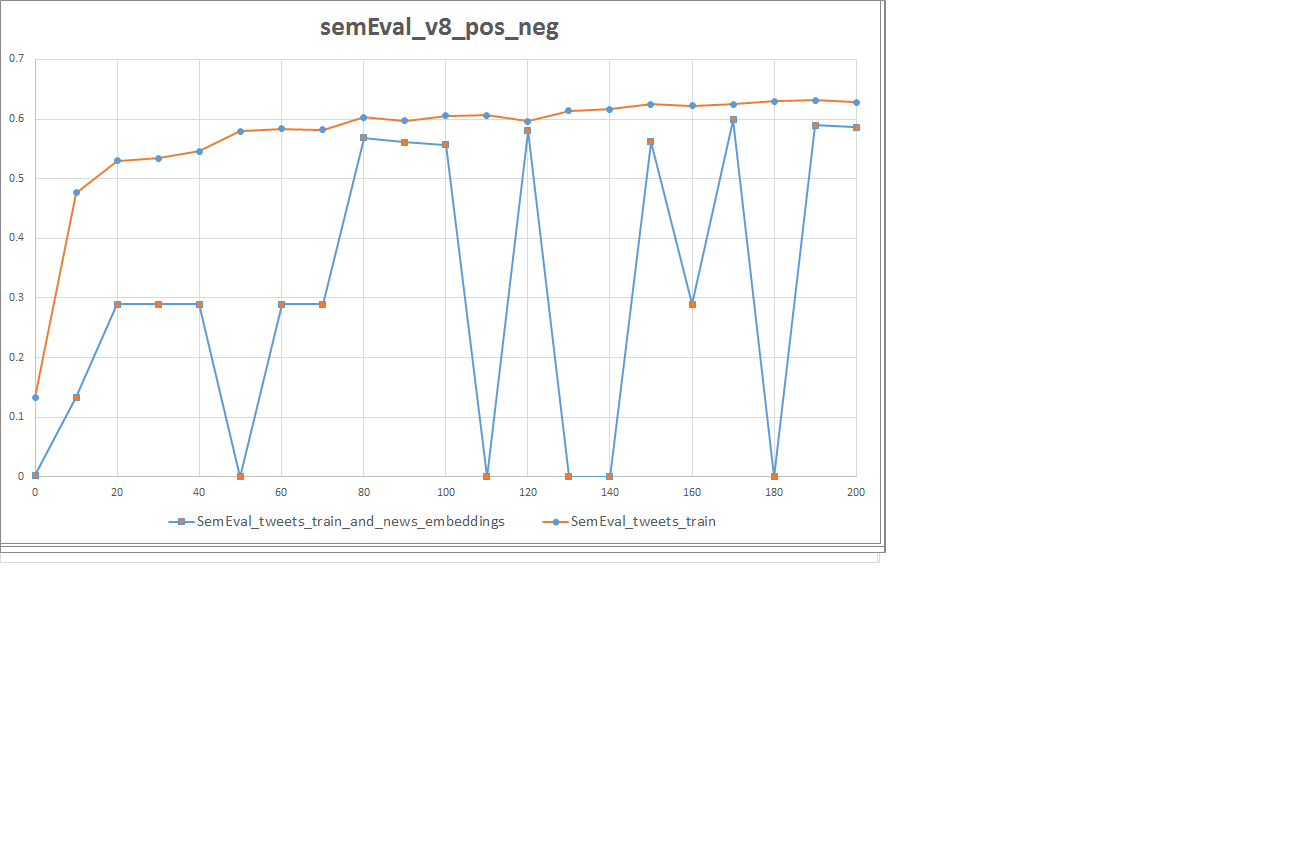
\includegraphics[width=0.49\textwidth]{img/Embeddings_V8_SemEval.png}}
	\caption{Word-Embeddings, F1 Score V8}
	\label{fig:Results V8}
\end{figure}

\begin{figure}[H]
	\centering
	\subfigure[V10 auf MPQ mit news Emeddings]{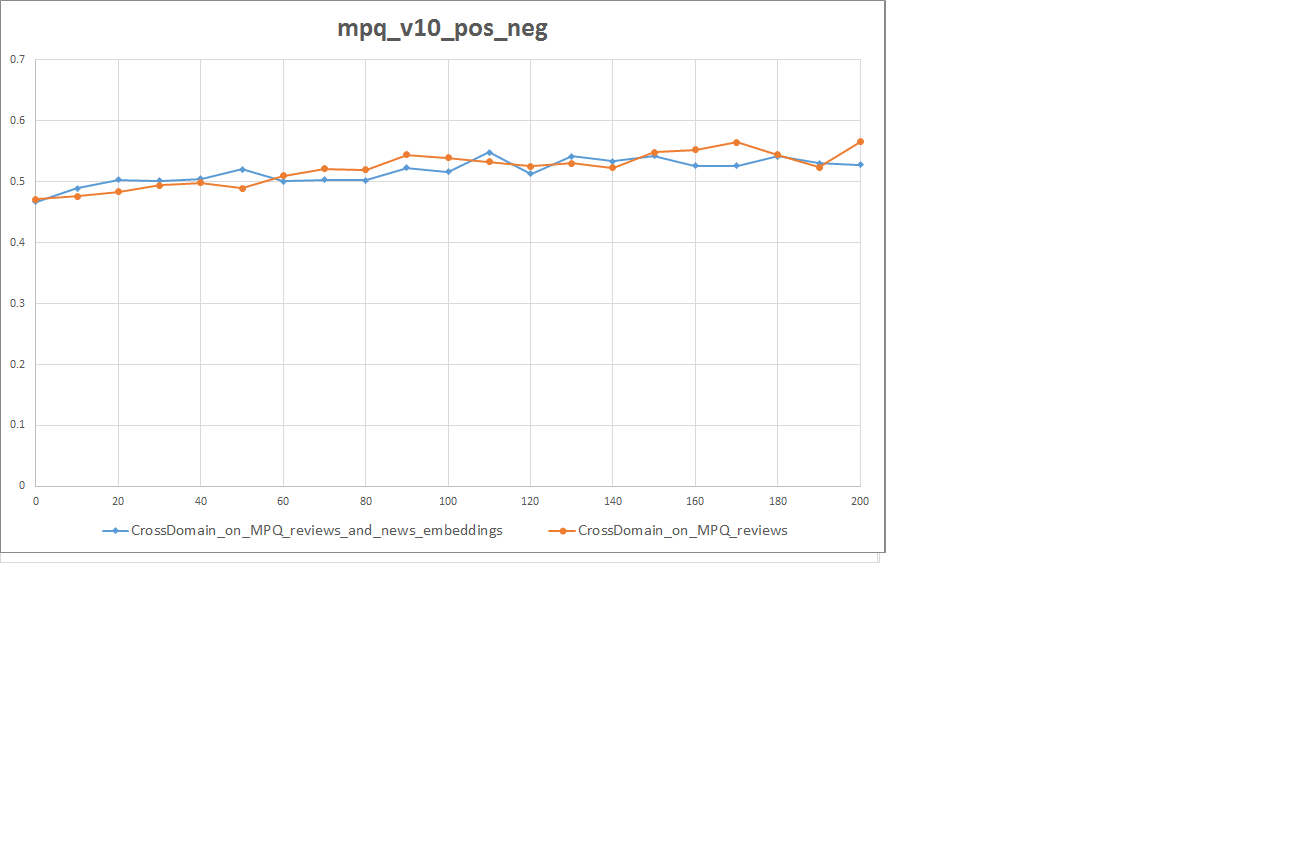
\includegraphics[width=0.49\textwidth]{img/Embeddings_V10_MPQ.png}}
	\caption{Word-Embeddings, F1 Score V10}
	\label{fig:Results V10}
\end{figure}

\begin{figure}[H]
	\centering
	\subfigure[V12 auf MPQ mit news Emeddings]{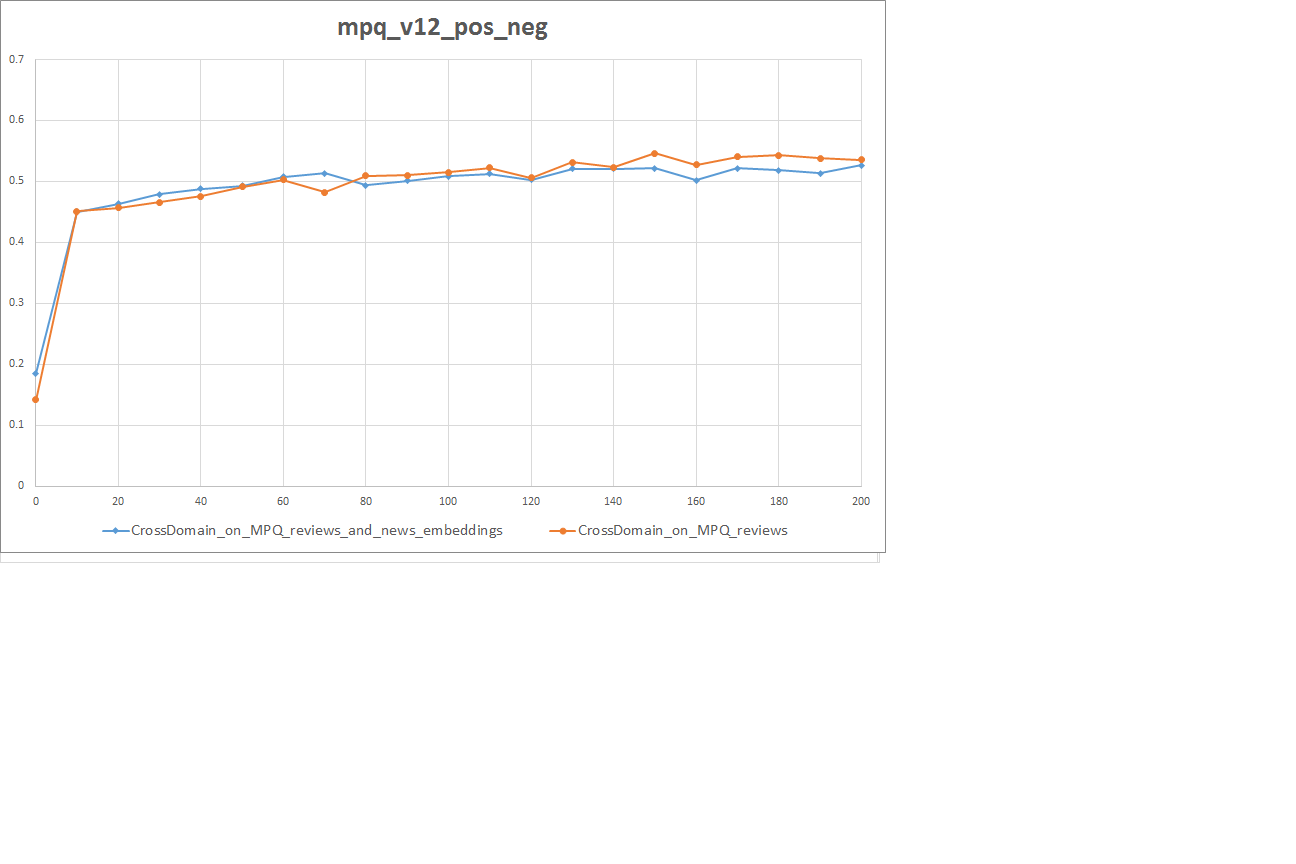
\includegraphics[width=0.49\textwidth]{img/Embeddings_V12_MPQ.png}}
	\subfigure[V12 auf SemEval mit tweets Emeddings]{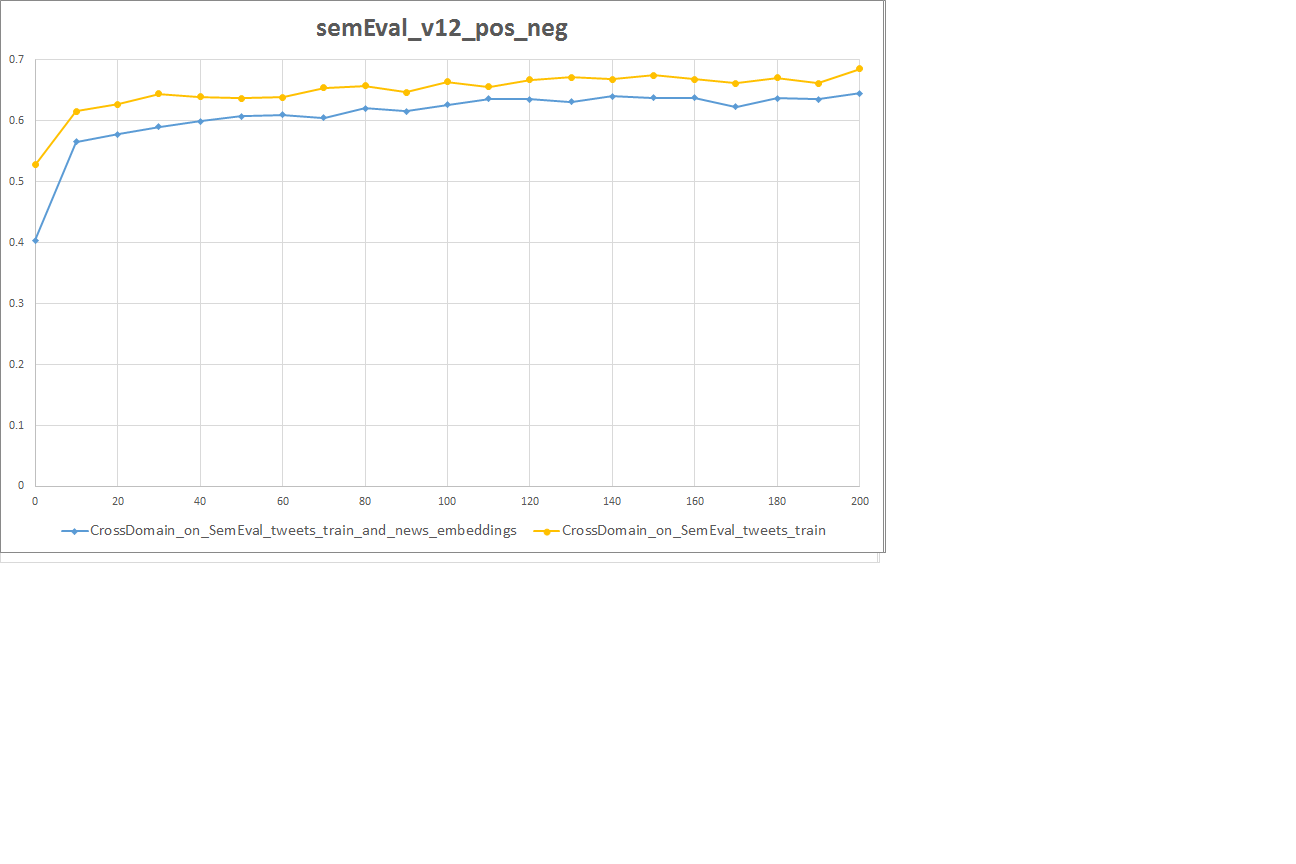
\includegraphics[width=0.49\textwidth]{img/Embeddings_V12_SemEval.png}}
	\caption{Word-Embeddings, F1 Score V12}
	\label{fig:Results V12}
\end{figure}